\chapter{RESULTS}
\thispagestyle{plain}

\label{Results}

In this chapter, I discuss experiments that test \fw for accuracy and computational efficiency.
These experiments also serve as examples of \fw being applied to a variety of ABMs.
In the next section, the different evaluation criteria are outlined.
Each of these metrics will be applied to a number of domains using a number of different techniques for the forward mapping.
The four domains used for the sake of experimentation were outlined in Chapter \ref{Domains}.
Each of these domains have unique properties that provide unique challenges to show the versatility of \fw.
The different regression methods for the forward mapping are outlined in Section \ref{sec:fmalgo}.
Finally, in Section \ref{sec:exps}, the statistical results are discussed.

\section{Evaluation}

Evaluating \fw is important because it shows that the framework is a practical and useful tool for studying ABMs.
Evaluation is split into two processes: evaluating the forward mapping solution and evaluating the reverse mapping solution.
Accuracy of these mappings in modeling the behavior space of the target ABM is paramount in importance.
If the forward and reverse mappings are not accurate, there would be no reason to use this framework for investigating behaviors of ABMs.
Computation time is also an important factor in evaluating \fw.
Interactions with the user need to be quick in order to make using \fw more convenient than manually inspecting the target ABM.
The response time of when a user interacts with \fw is the \textit{online} time and is far more important than the \textit{offline} time, the one-time computation requirement to learn the forward or reverse mapping.


 \subsection{Forward Mapping}

  \subsubsection{Accuracy}
Accuracy is the measurement of how closely the forward mapping represents the true behavior space of a target ABM.
To measure this, the difference (error) $\varepsilon$ between the predictions for a system level property $\hat y$ that the forward mapping produces and the actual value $y$ for a sampled point: $\varepsilon = |\hat y - y|$.
This measurement is performed many times for a single domain to produce the median error and the the upper and lower quartiles of the errors.

The errors are gathered by performing cross validation.
Two subsets of data points are randomly pulled from the master set of samples to create a training set and a validation set.
The forward mapping is built by using the training set, and then checked with the validation set.

The error is calculated for varying size data sets to show the relationship between error and data set size.

  \subsubsection{Offline Computation Time}

Offline computation time is the average amount of system time the forward mapping uses to train a model.
This is measured as the amount of time the pre-processing takes, given a training set.
The size of the training set is varied to determine how forward mapping training time is correlated to training set size.
Each forward mapping method is compared to the others.

  \subsubsection{Online Computation Time}

Online computation time is the average amount of time \fw takes to return the results of a user-submitted query.
This is measured by performing a large number of queries and calculating the average run time.
The size of the training set can affect the amount of time a query will take with some algorithms.
In these cases, the size of the training set is varied to determine how query time correlates to training set size.

 \subsection{Reverse Mapping}

  \subsubsection{Accuracy vs. Forward Mapping}
Accuracy of the reverse mapping is measured in two ways.
The first is how accurately the reverse mapping models the forward mapping.
Recall that \fw solves the reverse mapping by building an invertible approximation of the forward mapping.
This metric determines if this approach is doing what is expected to do.
The effect that granularity has on this accuracy is also measured by learning the same mapping with increasingly higher granularity.

\begin{figure}[ht]
\centering
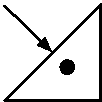
\includegraphics[scale=1]{images/mosterror.pdf}
\caption{The most erroneous spot in a right-angled simplex.}
\label{fig:mosterror}
\end{figure}

The error is presented as an ``average worst-case scenario".
The area of the reverse mapping space that is be the most erroneous is typically be the one furthest from the knots (corners of the simplex).
An illustration of this point is presented in Figure \ref{fig:mosterror}.
The point is halfway between all corners, except for the corner at the right angle.
This point is the most erroneous if the forward mapping is monotonically changing from one side of the simplex to the other (i.e., there are no local maxima or minima within the space).
Note that the reverse mapping will be identical to the forward mapping at the knots, since the forward mapping was used to infer their values.

Calculating the approximate upper bound on error, within a simplex, involves interpolating the system-level property value at the most erroneous point.
This is done by average the system-level property values of all corners not at the right angle.
Also, the location of the most erroneous point is queried for prediction through the forward mapping.
The difference between the interpolated value on the simplex and the actual predicted value using the forward mapping constitutes the error.
This metric is applied for every simplex and then averaged.
Thus, the metric measures the average error over all the worst-case scenarios for each simplex.
Also, the distribution of these errors is recorded to convey how consistent the reverse mapping is.


  \subsubsection{Accuracy vs. Agent-Based Model Run}

The main goal of the reverse mapping is to be able to suggest configurations that would generate a specified behavior.
This approach is different from the previous metric because it measures the difference between the reverse mapping and the true behavior space.

\begin{figure}[ht]
\centering
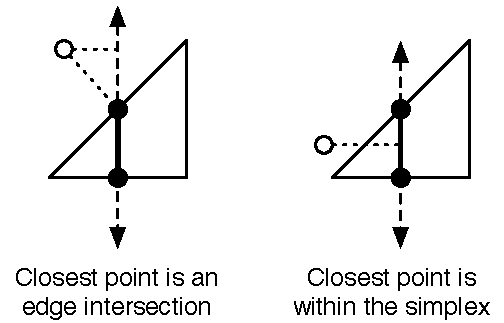
\includegraphics[scale=1]{images/closest.pdf}
\caption{Two cases for the closest point to a simplex intersection.}
\label{fig:closest}
\end{figure}

Error is measured by generating a random configuration point and sampling it from the agent-based model.
Then, the system-level property that was measured is passed to \fw to generate a reverse-mapping solution.
The error is the distance from the original configuration and the reverse-mapping solution space.
This value is calculated by adhering to the following procedure, per simplex:
\begin{enumerate}
  \item Determine the distance from the original point to the intersecting hyperplane.
  \item If the shortest line from the hyperplane to the point intersects the hyperplane \textit{within} the simplex, then the distance from the hyperplane is the distance from the intersection to the point.
  \item Otherwise, the closest point is one of the edge intersections.
\end{enumerate}
The two different cases (closest to an edge (left) and closest to the hyperplane (right)) are illustrated in Figure \ref{fig:closest}.
The minimum of all of these closest simplex points is taken as the distance from the actual system-level property value to the piecewise curve generated by the reverse mapping.


Several random configurations are sampled in this way.
The average and standard deviation of these errors are calculated to convey the accuracy of the reverse mapping, as well as the consistency of the reverse mapping.

  \subsubsection{Offline and Online Computation Time}
Offline computation time and online computation time is measured the same way for the reverse mapping as the forward mapping.
The amount of time \fw takes to prepare the reverse mapping is the offline computation time, and the amount of time required to produce a reverse mapping solution is the online computation time.



\section{Forward Mapping Methods}\label{sec:fmalgo}

For the experiments in this chapter, the three algorithms described in Chapter \ref{Background} are used for the forward mapping. In the following outline, I indicate specific configuration parameters or implementation details of importance.
\begin{itemize}
 \item k-nearest neighbor (KNN)
  \begin{itemize}
   \item Custom implementation with Python.
   \item 10-fold validation is used to determine the best $k$ out of a set of possible $k$ values.
  \end{itemize}

 \item robust locally weighted regression and smoothing scatterplots (LOESS)
  \begin{itemize}
   \item Custom implementation with Python.
   \item A good window is selected by myself for each domain. Changing this configuration parameter per sample size does not affect accuracy, as it does with kNN.
   \item Performs one smoothing operation. I found that increasing the number of smoothing operations past one provided limited improvement in accuracy and occasionally worsening accuracy. Finding an optimal smoothing with cross validation, per training set, would be computationally expensive.
  \end{itemize}

 \item nonlinear regression (NLR)
   \begin{itemize}
      \item Implemented in Python and uses the SciPy\footnote{SciPy is a freely available Python module that has a number of useful computational tools. The SciPy website is: http://www.scipy.org/} package to optimize the parametric model with least-squares.
   \end{itemize}

\end{itemize}


\section{Experiments}\label{sec:exps}

First, I will discuss results from the Fires domain together, which provides an extended example that explains the methodology and results for each of the seven experiments.
The rest of the experiments  for the other domains are grouped together by experiment, so that the effectiveness of the different components of \fw are evaluated independently.

 \subsection{Fires Domain Experiments}

The NetLogo Fires domain is an excellent example for showing how \fw works, as the domain is relatively simple and easy to visualize.
Plots of the behavior space for this domain are shown in Figure \ref{fig:rii}.


%training sizes of 20-200 (step 20)
% fm was trained 20 times per training set size
% 15 different validation sets were used on 15 different fm from different validation sets
% validation set size 2500
% granularities 25-300 (step 25)
% rm was retrained 15 times and validated with the 2500 points
% rm uses kNN with the highest data set size (200)


\subsubsection{Forward Mapping Training Time}


\begin{figure}[ht]
\centering
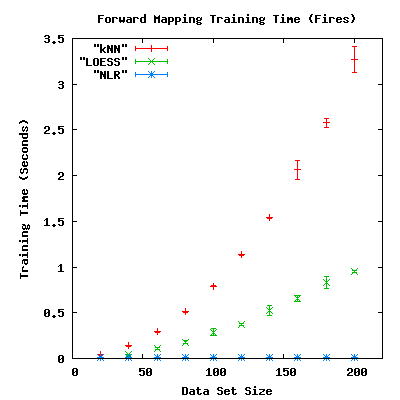
\includegraphics[scale=.5]{images/results_fires/fmtraining.png}
\caption{The average length of time required by the forward mapping to train.
The error bars show the 95\% confidence interval for the mean.}
\label{fig:fmtraining}
\end{figure}

Different training data set sizes, ranging from 20 to 200 (with a step of 20), were used to measure the amount of computation time the forward mapping requires to train a model.
Each of the three regressions were retrained twenty times per training data set size.
The results are plotted in Figure \ref{fig:fmtraining}.
This plot shows that kNN grows faster than the other two approaches with increasing data set sizes.
This is because the 10-fold validation for picking $k$ requires a significant amount of time.
Meanwhile, LOESS grows at a linear rate.
The training time for NLR is insignificant in comparison to the other approaches.
Least-squares optimization is a mature subject area, and SciPy uses some of the most advanced methods to make the optimization quick.

Even the slowest of these regressions, kNN with 200 training instances, runs in only 3.25 seconds, which is acceptable for a one-time process.


The error bars show that there is little variability in training time, meaning that the approaches are consistent in the amount of time they take.


\subsubsection{Forward Mapping Accuracy}

\begin{figure}[ht]
\centering
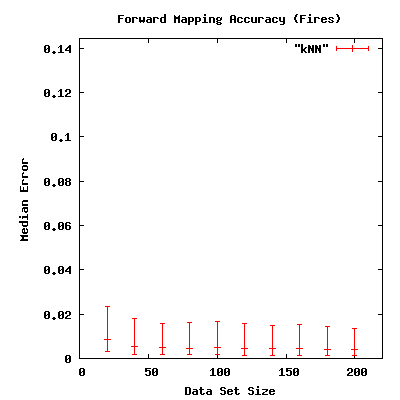
\includegraphics[scale=.3333333]{images/results_fires/fmacc-kNN.png}
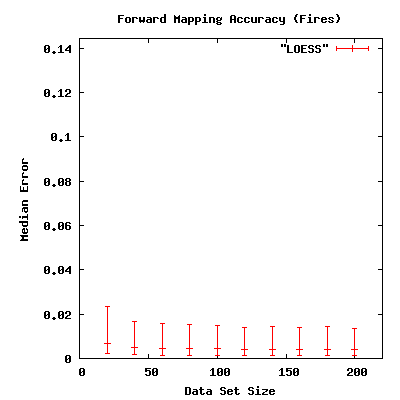
\includegraphics[scale=.3333333]{images/results_fires/fmacc-LOESS.png}
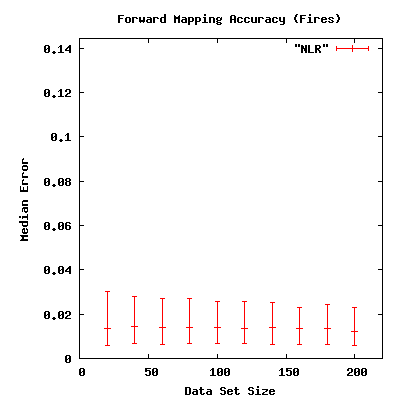
\includegraphics[scale=.3333333]{images/results_fires/fmacc-NLR.png}
\caption{...}
\label{fig:fmacc}
\end{figure}

Different training data set sizes, ranging from 20 to 200 (with a step of 20), were used to train a model.
Fifteen different training data sets were produced per data set size.
For each of these trained models, 2500 points from a validation set were used to evaluate the accuracy of the forward mapping, in respect to values sampled directly from ABMs.
The configuration of each validation instance was passed into the forward mapping to retrieve a predicted value.
This predicted value was then compared to the sampled value from the validation instance to produce an error value.

The accuracy of the forward mapping is very high, for all three approaches: all three approaches predict the amount of trees burned down within an accuracy of 1\%.
The median error, along with the upper quartile and lower quartile are plotted in Figure \ref{fig:fmacc}.

This is impressive considering to the amount of variability from sample to sample of the Fires domain.
Both KNN and LOESS perform better with more data points, however with a sample size greather than 80, the accuracy does not appear affected very much.
Overall, KNN had a lower median error than LOESS, but not by a statistically significant amount.
NLR performed worse than the other two approaches and experienced more variance in its errors.
Interestingly, the accuracy of NLR only slightly improved from a data sample size of 20 to a data sample size of 200.
Since NLR is a parametric approach, the optimal model for a small number of points will be very similar to the optimal model for a large number of points from the same distribution.
Meanwhile, locally weighted nonparametric approaches have the ability to fit sections of the behavior space more closely as more points are provided.
This trade off is demonstrated in the accuracy results.


\subsubsection{Forward Mapping Query Time}
\begin{figure}[ht]
\centering
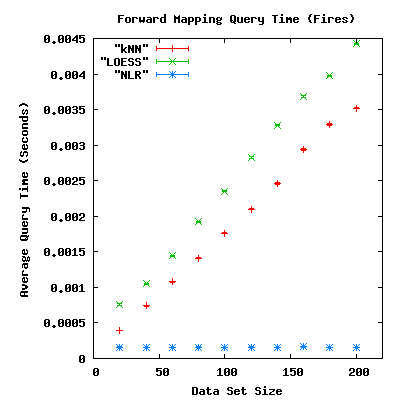
\includegraphics[scale=.5]{images/results_fires/fmquery.png}
\caption{...}
\label{fig:fmquery}
\end{figure}

Measurements of the query time were performed at the same time as the accuracy measurements.
The elapsed time was measured for every prediction call to the forward mappings.

Queries to the forward mappings for the three approaches are fast.
The longest time for a query to execute was .0045 seconds for LOESS using a data set of size 200.
This amount of time is instantaneous to a human user and thus satisfies the requirement that the forward mapping is fast for the user.
As expected, data set size has no effect on the computation time of NLR because the model equation is always the same number of parameters.
Also, as expected, LOESS and kNN query time grows linearly with the size of the data set.
For every new point added, an additional point must be checked to see if it is local to the passed in configuration, or not.


\subsubsection{Reverse Mapping Training Time}

\begin{figure}[ht]
\centering
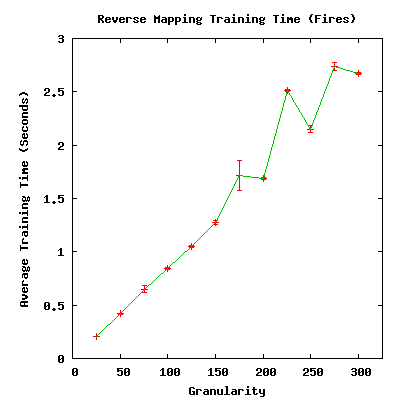
\includegraphics[scale=.5]{images/results_fires/rmtraining.png}
\caption{...}
\label{fig:rmtraining}
\end{figure}

The most accurate forward mapping trained in the previous forward mapping experiments was used for the reverse mapping experiments.
In this case, I used kNN with a training set of 200.
Training time was measured for reverse mappings training on granularities of 25 to 300 (step 25).
A granularity of $N$ means the configuration space was split into $N$ simplexes, per dimension.
The test was repeated fifteen times per granularity.

The training time increased linearly with an increase in granularity.
With a granularity of three hundred, the training time was under three seconds.
With a granularity of twenty-five, the training time was just under a quarter of a second.


\subsubsection{Reverse Mapping Accuracy}

\begin{figure}[ht]
\centering
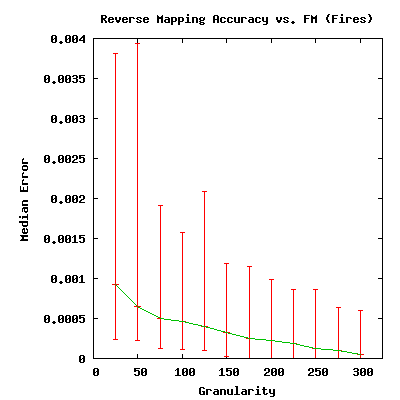
\includegraphics[scale=.5]{images/results_fires/rmaccfm.png}
\caption{...}
\label{fig:rmaccfm}
\end{figure}

The reverse mapping accuracy is measured in two ways.
First, I measured the median error of the reverse mapping in respect to the predicted values of the forward mapping.
This metric demonstrates the accuracy of fifteen different reverse mappings per granularity, as an approximation of the forward mapping.
This metric is measured by taking each simplex in the reverse mapping and selecting the furthest point from the corners.
Each of these points are then passed to the forward mapping to provide a prediction, which is then compared to the interpolated value within the simplex.
The difference between these two denote the error of the values within the simplex, in respect to the forward mapping it is approximating. 

Figure \ref{fig:rmaccfm} shows the effect of granularity on median error.
The error steadily decreases with higher granularity, eventually approaching 100\% for about half of the queries.
Also, the error is extremely low in all cases, never exceeding half a percent of trees burned down.
The reverse mappings trained with high granularities were often accurate within a tenth of a percent of trees burned down.

\begin{figure}[ht]
\centering
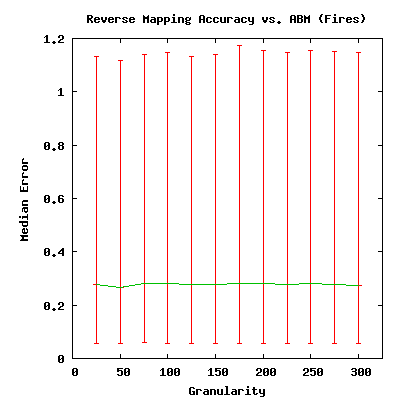
\includegraphics[scale=.5]{images/results_fires/rmaccabm.png}
\caption{...}
\label{fig:rmaccabm}
\end{figure}
The second way the accuracy of the reverse mapping is measured is how distant the piecewise configuration curve returned by the reverse mapping is from the actual configuration.
Recall that the reverse mapping returns a set of intersections (however, in the case of Fires typically only one, since the mapping is one-to-one).
This metric intends to measure the distance from a configuration suggested by the reverse mapping, and the actual configuration from the validation set.
Each of the 2500 instances from the validation set were used for each of the reverse mappings that were trained.

The results in Figure \ref{fig:rmaccabm} show that the median error remains fairly constant, regardless of granularity.
The reason for this is that the error incurred by the approximation of the forward mapping is insignificant in comparison to the error of kNN.
Since the same kNN forward mapping was used for all granularities, the error incurred by the reverse mapping is not noticeable or statistically significant.


\subsubsection{Reverse Mapping Query Time}

\begin{figure}[ht]
\centering
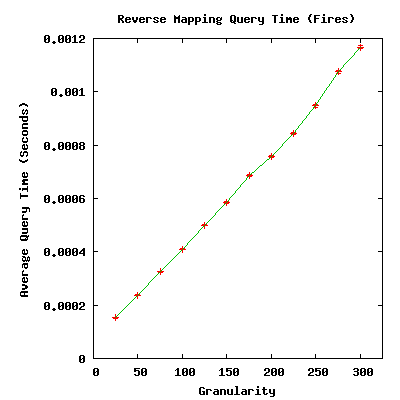
\includegraphics[scale=.5]{images/results_fires/rmquery.png}
\caption{...}
\label{fig:rmquery}
\end{figure}

The reverse mapping query time was measured along with the accuracies of the reverse mapping, in respect to the validation set.

Overall, the average reverse mapping query computation time is almost instantaneous, taking about 0.0012 seconds with a granularity of 300, as seen in Figure \ref{fig:rmquery}.
The average query time increased linearly with the granularity because each additional simplex must be checked for intersections.


 \subsection{Forward Mapping}

  \subsubsection{Accuracy}

\begin{figure}[ht]
\centering
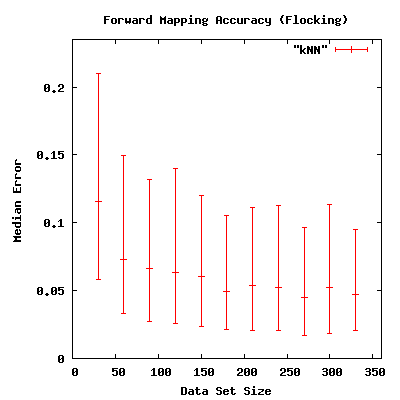
\includegraphics[scale=.4]{images/results_flocking/fmacc-kNN.png}
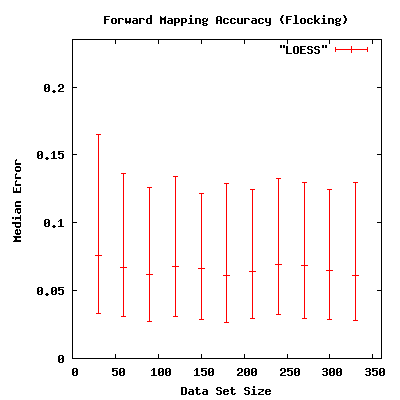
\includegraphics[scale=.4]{images/results_flocking/fmacc-LOESS.png}
\caption{...}
\label{fig:flockfmacc}
\end{figure}

Figure \ref{fig:flockfmacc}.

\begin{figure}[ht]
\centering
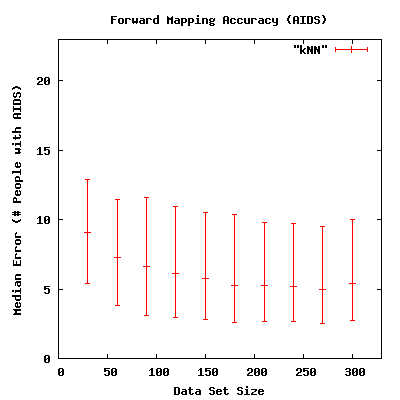
\includegraphics[scale=.5]{images/results_aids/aids-fmacc.png}
\caption{...}
\label{fig:aidsfmacc}
\end{figure}

Figure \ref{fig:aidsfmacc}.


  \subsubsection{Offline Computation Time}

\begin{figure}[ht]
\centering
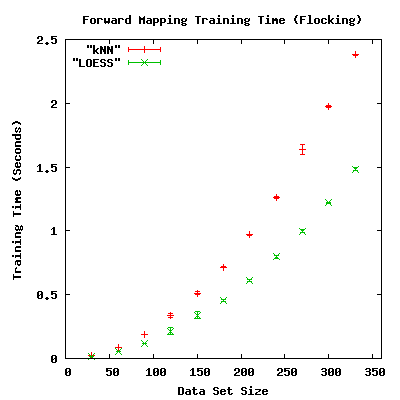
\includegraphics[scale=.4]{images/results_flocking/fmtraining.png}
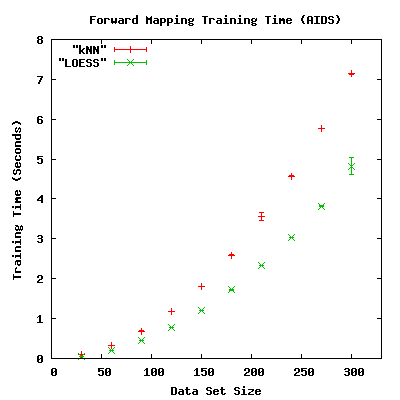
\includegraphics[scale=.4]{images/results_aids/aids-fmtraining.png}
\caption{...}
\label{fig:flockfmtraining}
\end{figure}

Figure \ref{fig:fmtraining}.




  \subsubsection{Online Computation Time}

\begin{figure}[ht]
\centering
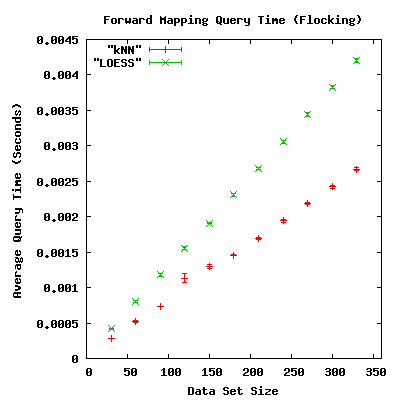
\includegraphics[scale=.4]{images/results_flocking/fmquery.png}
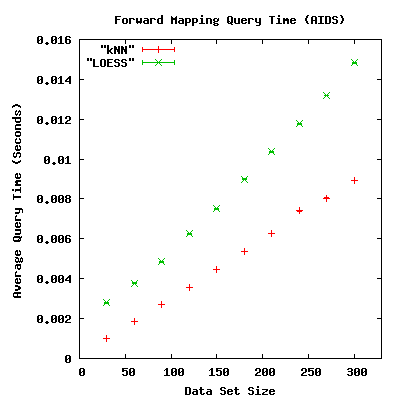
\includegraphics[scale=.4]{images/results_aids/aids-fmquery.png}
\caption{...}
\label{fig:flockfmquery}
\end{figure}

Figure \ref{fig:fmquery}.


 \subsection{Reverse Mapping}

  \subsubsection{Accuracy vs. Forward Mapping}

\begin{figure}[ht]
\centering
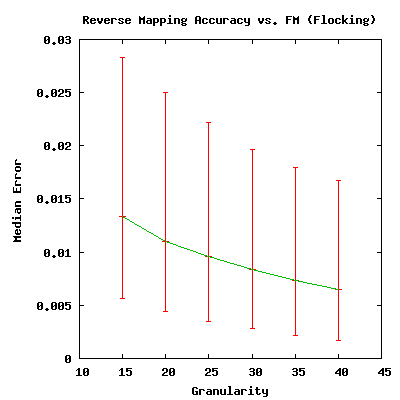
\includegraphics[scale=.5]{images/results_flocking/rmacc.png}
\caption{...}
\label{fig:flockrmacc}
\end{figure}

Figure \ref{fig:flockrmacc}.

  \subsubsection{Accuracy vs. System Run}

  \subsubsection{Offline Computation Time}

\begin{figure}[ht]
\centering
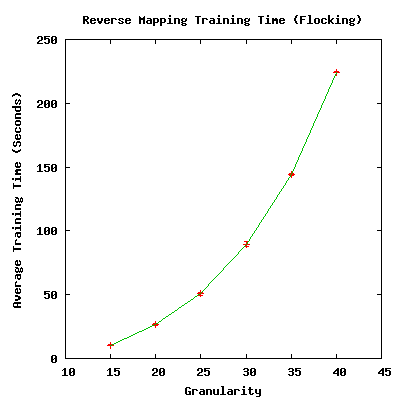
\includegraphics[scale=.5]{images/results_flocking/rmtraining.png}
\caption{...}
\label{fig:flockrmtraining}
\end{figure}

Figure \ref{fig:flockrmtraining}.

  \subsubsection{Online Computation Time}

\begin{figure}[ht]
\centering
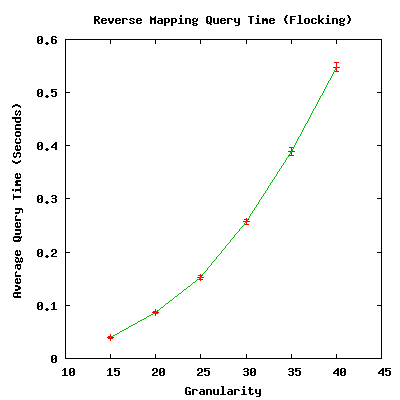
\includegraphics[scale=.5]{images/results_flocking/rmquery.png}
\caption{...}
\label{fig:flockrmquery}
\end{figure}

Figure \ref{fig:flockrmquery}.




